%!TEX root = ../main.tex

\section{Постановка задачи}

\begin{frame}{Математическая модель}
\begin{block}{Модель типа диффузной границы}
	Вещество находится в разных фазах. Состояние вещества описывается гладкой функцией $\phi(\vx, t)$ -- фазовым полем.
\end{block}
\begin{itemize}
	\item $\phi = 1$ -- неповрежденная среда
	\item $\phi = 0$ -- полностью разрушенная среда
	\item Зона $\phi \in (0, 1)$ -- диффузная граница
	\item На разрушение среды тратится энергия
\end{itemize}
\begin{figure}
	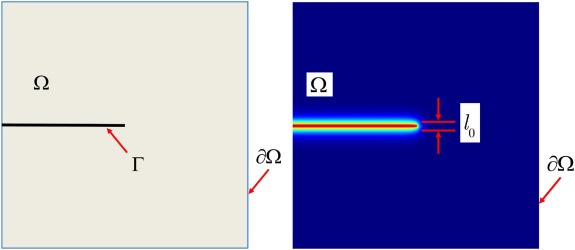
\includegraphics[width=0.5\textwidth]{figures/diffuse_edge.jpg}
\end{figure}
\end{frame}


\begin{frame}{Математическая модель}
%\vspace{-0.3cm}
\begin{block}{Уравнения динамики системы}
	\begin{gather*}
		\Div(\epsilon[\phi] \nabla \Phi) = -\rho_E \\
		\partt{\rho_E} = \Div(\sigma[\phi] \nabla \Phi) \\
		\cfrac{1}{m} \partt{\phi} = -F'( \phi; \| \nabla \Phi \|) + \cfrac{\Gamma}{2} \Delta \phi + \beta \Gamma l^2 \Div \left( \| \nabla \phi \|_2^2 \nabla \phi \right)
	\end{gather*}
\end{block}
\begin{itemize}
	\item Плотность свободной энергии Гельмгольца
	\vspace{-0.2cm}
	\[
		\pi = F( \phi; \| \nabla \Phi \|) + \cfrac{\Gamma}{4} \| \nabla \phi \|_2^2 + \cfrac{\beta}{4} \Gamma l^2 \| \nabla \phi \|_2^4
	\]
	\item $m$, $\Gamma$, $l$ -- параметры модели, константы
\end{itemize}
\end{frame}


\begin{frame}{Математическая модель}
\begin{gather*}
	F(\phi; \| \nabla \Phi \|) = -\half \epsilon[\phi] \cdot \| \nabla \Phi \|_2^2 + \Gamma \cfrac{1 - f(\phi)}{l^2} \\
	\begin{alignedat}{3}
		\epsilon[\phi] &= \epsilon(\vx, t) &&= \cfrac{\epsilon_0(\vx)}{f(\phi(\vx, t)) + \delta} \\
		\sigma[\phi] &= \sigma(\vx, t) &&= \cfrac{\sigma_0(\vx)}{f(\phi(\vx, t)) + \delta}
	\end{alignedat} \\[2mm]
	f(\phi) = 4 \phi^3 - 3 \phi^4
\end{gather*}
\vspace{-3mm}
\begin{itemize}
	\item $\delta$ -- регуляризующий параметр
	\item $f(\phi)$ -- интерполирующая функция
\end{itemize}
\end{frame}


\begin{frame}{Разностная схема}
\vspace{-5mm}
\begin{enumerate}
	\item $\; \Div_h \left( \epsilon[\phi] \nabla_h \hat{\Phi} \right) = - \rho_E \quad \leadsto \quad \hat{\Phi}$
	\item $\left[ \partt{\phi} \right]_h = m \cdot \left( -F'( \phi; \| \nabla_h \hat{\Phi} \|) + \cfrac{\Gamma}{2} \Delta_h \phi + \beta \Gamma l^2 \Div_h \left( \| \nabla_h \phi \|_2^2 \nabla_h \phi \right) \right)$
	\item $\left[ \partt{\rho} \right]_h = \Div_h \left( \sigma[\phi] \nabla_h \hat{\Phi} \right)$
	\item $\hat{\phi} = \phi + \tau \cdot \left[ \partt{\phi} \right]_h; \qquad \hat{\rho}_E = \rho_E + \tau \cdot \left[ \partt{\rho} \right]_h$
\end{enumerate}
\end{frame}


\begin{frame}{Цель работы}
\vspace{-3mm}
\begin{center}
\begin{minipage}{0.95\textwidth}
\begin{block}{Цель работы}
	Исследовать применение адаптивного шага по времени при расчете задачи в полной, трехмерной постановке
\end{block}
\end{minipage}
\end{center}
\vspace{3mm}
\hspace{8mm} Требования к алгоритму адаптации:
\begin{itemize}
	\item Простота реализации
	\item Малый объем дополнительных вычислений
\end{itemize}
\end{frame}